\documentclass[10pt]{article}
\usepackage[T1]{fontenc}
\usepackage[english]{babel}
\usepackage[a4paper,head=15pt,body={17cm,25cm},top=2.5cm]{geometry}
\usepackage{amsmath,amssymb}
\usepackage{graphicx}
\usepackage{float}
\usepackage{booktabs}
\usepackage{tikz}
\usepackage{algorithm}
\usepackage{algpseudocode}
\usepackage{cite}
\usepackage{titlesec}
\usepackage{fancyhdr}
\usepackage{hyperref}

% Section titles: bold, normal size
\setlength{\columnsep}{3em}
\titleformat{\section}{\normalfont\bfseries}{\thesection}{2ex}{}
\titlespacing*{\section}{0pt}{2.5ex}{1ex}
\titleformat{\subsection}{\normalfont\bfseries}{\thesubsection}{2ex}{}
\titlespacing*{\subsection}{0pt}{2.5ex}{1ex}
\setlength{\abovecaptionskip}{0pt}
\setlength{\belowcaptionskip}{0pt}

\newtheorem{definition}{Definition}
\newtheorem{theorem}[definition]{Theorem}

% Header and footer
\pagestyle{fancy}
\fancyhf{}
\fancyhead[R]{\bfseries\thepage}
\fancyhead[L]{\bfseries CSCI 6360: Parallel Computing, Final Project}
\renewcommand{\headrulewidth}{0.5pt}
\renewcommand{\footrulewidth}{0.5pt}
\fancypagestyle{plain}{\fancyhead{}}

\begin{document}

\twocolumn[
  \begin{center}
    \bfseries Parallel Solver for Poisson's Equations in Two Dimensions
    \bigskip

    Ngan Le
    \smallskip

    \mdseries Department of Mathematical Sciences, Rensselaer Polytechnic Institute, Troy, NY 12180, USA
  \end{center}
]

\section*{Abstract}
We develop a parallel solver for Poisson's equations in two dimensions. The methods are based on the Successive Over-Relaxation (SOR($\omega$)) techniques, which iteratively solve the linear system derived from the spatial discretization using finite difference approximation of the Poisson problem.
The method divides the points on the grid into red and black points. The grid points of the same color can be updated in parallel without conflicting with each other because they are independent of each other. Thus, at each iteration, the SOR($\omega$) method updates all the red grid points in one step, and then updates all the black points in the second step. 
This approach offers a great way for parallelism using the MPI and CUDA frameworks, since the computation at each iteration can be done in parallel effectively. 
Numerical results are illustrated, including solver verification, weak scaling, strong scaling, and runtime analysis in parallel using MPI and CUDA, demonstrating the potential of the parallel solvers for large-scale problems in scientific computing.

\smallskip

\noindent\textbf{Keywords:} Poisson equation, finite difference approximation, SOR($\omega$) methods. 
\section{Introduction}
%Helmholtz problems often arise in many applications in science and engineering, including acoustics, electromagnetic scattering, medical imaging, geophysical modeling, seismics, $\dots$. \\
Poisson's equation is a class of elliptic partial differential equations. These equations often arise in a variety of fields in science and engineering, with their applications ranging from electrostatics, fluid dynamics, and thermodynamics, among others. 
Thus, designing an effective solver for Poisson's equation is a crucial task for a wide range of fundamental applications. In this project, we implement the parallel solver for Poisson's equation in two dimensions. The solver is based on the finite difference method \cite{leveque} by first discretizing the domain problem using central second-order approximations, leading to a large but sparse linear system. Then the resulting linear system is solved iteratively using SOR($\omega$) methods with the red-black ordering \cite{adams1988,young1954,zhang1996}. This ordering gives an advantageous method in which the grid points are updated, in the sense that updating the grid nodes only involves the black points and vice versa. Consequently, each iteration involves one step of updating red nodes, followed by another step of updating black points, and due to the independence, each update can be done in parallel. The parallel solvers are developed using MPI and CUDA platforms. Numerical results are presented demonstrating the algorithm showing the substantial speedups and scalability for the problems in two dimensions. In particular, for certain problem sizes, we can gain up to $27\times$ speedups compared to that of serial solvers.

There has been a wide range of solvers developed for solving Poisson's equation as well as elliptic equations in general. On the one hand, the resulting discretized linear system resulting from the spatial discretization can be solved by direct methods based on sparse factorization, including sparse LU, Cholesky \cite{hackbusch1994, saad2003}. However, the methods are limited as the problem sizes grow, especially for problems in three dimensions because of the fill-ins leading to the requirement for a significant amount of storage. Hence, for large-scale problems, iterative methods are favored over direct methods. Classical iterative methods such as Jacobi's, Gauss-Seidel, and SOR, which are discussed in Section~\ref{sec:methods}, are one of the simplest approaches for solving linear systems. Despite their simplicity, these methods are essential in more advanced methods. For example, they are used as relaxation schemes in multigrid methods \cite{brandt1977,briggs2000}, and as preconditioners for GMRES \cite{trefethen1997,trottenberg2001} and domain decomposition methods \cite{smith1996}. Alternatively, Poisson's equation can be solved directly based on fast Fourier transform \cite{cooley1965,hockney1988}. Depending on the problem's geometries, some of the methods can be advantageous over the others. A good comparision of these methods is given in \cite{gholami2016}. 

The remainder of the project is organized as follows. Section~\ref{sec:model} introduces the model problem and the numerical scheme  used to approximate it. Next, in Section~\ref{sec:methods}, we discuss some of the basic iterative solvers on which we build parallel solvers, as well as summarize their convergence properties. The numerical results of the model problems are presented in Section~\ref{sec:results}.
\section{Model and Numerical Approximations}\label{sec:model}
We are interested in finding the solution to Poisson's equation
{%\small
\begin{subequations}
\label{eq:poisson2d}
    \begin{align}
    & \dfrac{\partial^2 u}{\partial_x^2}+\dfrac{\partial^2 u}{\partial_y^2} = f(x,y), \quad (x,y) \in \Omega, \label{eq:poisson2dA}\\
    & u(x,y)= g(x,y), \qquad \quad \;  (x,y) \in \partial \Omega, \label{eq:poisson2dB}
\end{align}
\end{subequations}
}
where $\Omega$ is a bounded domain in $\mathbb{R}^2$ and $g(x,y)$ is some given function. For simplicity, the domain $\Omega$ is taken to be a unit square, i.e., $\Omega = [0,1]\times [0,1]$, and the values of $u$ at the boundary are taken to be zero, i.e. $g=0$.

We solve the problem using a finite difference approximation. The domain is discretized into grid points $(x_i, y_j)$ with $x_i = ih$ and $y_j=jh$, with 
$h=1/(N+1)$, where $N+1$ is the number of grid cells in each direction (so there will be total of $N+2$ points in each direction). Figure \ref{fig:2dGrid} shows an example of the domain $\Omega$ and a discretization of its domain.

\begin{figure}[htb]
 %\centering
 \begin{center}
    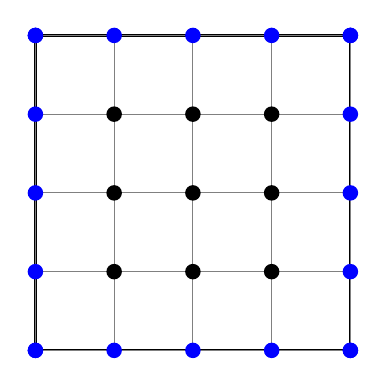
\begin{tikzpicture}[scale=4]

    \draw[thick] (0,0) rectangle (1,1);
    \draw[step=0.25, gray, thin] (0,0) grid (1,1);

    % Interior points
    \foreach \x in {0.25,0.5,0.75}
        \foreach \y in {0.25,0.5,0.75}
            \fill[black] (\x,\y) circle (0.7pt);

    % Boundary points
    \foreach \x in {0,0.25,...,1}
        \foreach \y in {0,1}
            \fill[blue] (\x,\y) circle (0.7pt);

    \foreach \y in {0,0.25,...,1}
        \foreach \x in {0,1}
            \fill[blue] (\x,\y) circle (0.7pt);

\end{tikzpicture}
\end{center}
 \caption{Uniform grid on the unit square, where boundary points are shown in blue and interior points in black.}  \label{fig:2dGrid}
\end{figure}
Let $u_{ij}=u(x_i, y_j)$ and $f_{ij}=f(x_i,y_j)$ then we can approximate the second derivatives in equation~\eqref{eq:poisson2dA} using second-order central approximations
\begin{subequations}
    \begin{align}
        & \dfrac{\partial^2 u}{\partial_x^2}\Big|_{x=x_i, y=y_j} \approx \dfrac{u_{i+1,j}-2u_{i,j} + u_{i-1,j} }{h^2}, \\
        & \dfrac{\partial^2 u}{\partial_y^2}\Big|_{x=x_i, y=y_j} \approx \dfrac{u_{i,j+1}-2u_{i,j} + u_{i,j-1}}{h^2}.
    \end{align}
\end{subequations}
From these approximations, we can approximate~\eqref{eq:poisson2dA} as
{\small  
\begin{align}
    & \dfrac{u_{i+1,j}-2u_{i,j} + u_{i-1,j} }{h^2} + \dfrac{u_{i,j+1}-2u_{i,j} + u_{i,j-1}}{h^2} = f_{ij}.
\end{align}
}
Or in a compact form,
\begin{align}
    u_{i+1,j}+u_{i-1,j} - 4u_{i,j} + u_{i,j+1}+u_{i,j-1} = h^2 f_{ij}.\label{eq:discreteEqn}
\end{align}
This holds for $i=1,2,\cdots, N$ and $j=1,2,\cdots,N$. This is called a \textit{$5$-point stencil} approximation, giving the second-order accurate approximation \cite{leveque} to the problem in~\eqref{eq:poisson2d}. Each equation involves 5 points, as illustrated in Figure\ref{fig:stencil}.
\begin{figure}[htb]
\begin{center}
    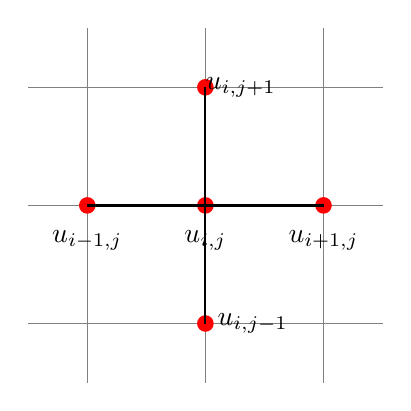
\begin{tikzpicture}[scale=1.5]
    
        % Draw grid
        \draw[step=1, gray, thin] (-1.5,-1.5) grid (1.5,1.5);
    
        % Central point
        \fill[red] (0,0) circle (2pt);
        \node at (0,-0.3) {$u_{i,j}$};
    
        % Neighboring points
        \fill[red] (-1,0) circle (2pt);
        \node at (-1,-0.3) {$u_{i-1,j}$};
    
        \fill[red] (1,0) circle (2pt);
        \node at (1,-0.3) {$u_{i+1,j}$};
    
        \fill[red] (0,1) circle (2pt);
        \node at (0.3,1) {$u_{i,j+1}$};
    
        \fill[red] (0,-1) circle (2pt);
        \node at (0.4,-1) {$u_{i,j-1}$};
    
        % Optional: draw connections
        \draw[thick] (0,0) -- (1,0);
        \draw[thick] (0,0) -- (-1,0);
        \draw[thick] (0,0) -- (0,1);
        \draw[thick] (0,0) -- (0,-1);
    
    \end{tikzpicture}
    \end{center}
    \caption{The 5-point stencil for a second-order finite difference approximation of the 2D Poisson equation} \label{fig:stencil}
\end{figure}

From the boundary conditions, we know $u_{0,j}=u_{N+1,j} = u_{i,0}=u_{i,N+1}$. Thus, the equation\eqref{eq:discreteEqn} defines a set of $n=N^2$ linear equations for the $n$ unknowns $u_{ij}$ for $i,j=1,2,\cdots,N$. The collection of these equations can be assembled into a large-sparse matrix equation of the form
\begin{align}
    \mathbf{Ax}=\mathbf{b}, \label{eq: matrixSystem}
\end{align}
where $\mathbf{x}$ is the vector containing all the unknonws $u_{ij}$ and $\mathbf{b}$ is the vector holding $f_{ij}$.
One method for solving the matrix system in~\eqref{eq: matrixSystem} is simply to use a sparse matrix solver. This is manageable when the problem is not large. However, for large-scale problems, especially problems in 3D, direct methods can be disadvantageous due to the fill-ins, and they require significantly more storage. Thus for large-scale problems, iterative methods are preferred over direct methods. There have been various methods developed for solving the large-scale linear systems. Our focus in this project is the SOR methods. The methods give a fundamental understanding for more advanced methods that can be used later.
The time and space complexity of some direct and iterative solvers are summarized in Table~\ref {tab:summarySolvers} (see \cite{demmel1993,demmel1997} for more details).

\begin{table}[htb]
%\begin{center}
% \centering
\small
% \setlength{\tabcolsep}{2.5pt}
\renewcommand{\arraystretch}{1.2} % row spacing

\begin{tabular}{l c c c c}
\toprule
\textbf{Method} & \textbf{Time} & \textbf{Space} & \textbf{D/I}  \\
\midrule

Dense Cholesky            & $n^3$       & $n^2$           & D  \\
Explicit inverse          & $n^2$       & $n^2$           & D         \\
Band Cholesky             & $n^2$       & $n^{3/2}$       & D  \\

\midrule
Jacobi                    & $n^2$       & $n$             & I  \\
Gauss--Seidel             & $n^2$       & $n$             & I \\
Sparse Cholesky           & $n^{3/2}$   & $n \log n$      & D \\

\midrule
Conjugate gradients       & $n^{3/2}$   & $n$             & I \\
SOR($\omega$)             & $n^{3/2}$   & $n$             & I \\
%SSOR with Chebyshev accel.& $n^{5/4}$   & $n$             & I \\

\midrule
Fast Fourier transform    & $n \log n$  & $n$             & D \\
Block cyclic reduction    & $n \log n$  & $n$             & D \\
Multigrid                 & $n$         & $n$             & I \\

\midrule
Lower bound               & $n$         & $n$             &   &      \\

\bottomrule

\end{tabular}
\vspace{6pt}
\caption{Order of complexity of solving Poisson’s equation on an $N$-by-$N$ grid
($n= N^2$). D/I here stand for \textit{direct solver} and \textit{iterative solver} respectively.}
%\end{center}
\label{tab:summarySolvers}
\end{table}

\section{Basic Iterative Methods}\label{sec:methods}
In this section, we discuss the most classical iterative methods for solving the linear system of the form $\mathbf{Ax=b}$. We will start with the Jacobi method then the Gauss-Seidel and finally talk about the SOR($\omega$) methods. Then we will discuss how to apply these methods to the model problem in~\eqref{eq:poisson2d}.

Given $\mathbf{x}^{(0)}$ is some initial guess, these methods generate a sequence $\mathbf{x}^{(m)}$ conveging to the solution $\mathbf{A^{-1}b}$ of $\mathbf{Ax=b}$, where $\mathbf{x}^{(m+1)}$ is cheap to compute form $\mathbf{x}^{m}$.
\begin{definition}
    A splititing of $\mathbf{A}$ is a decomposition of the form $\mathbf{A=M-K}$, where $\mathbf{M}$ is non-singular.
\end{definition}

Given a splitting of matrix $\mathbf{A}$ then the linear system becomes
\begin{align}
    \mathbf{(M-K)Ax=b},
\end{align}
which implies
\begin{align}
    \mathbf{Mx=Kx+b}.
\end{align}
Thus, it follows that
\begin{align}
    \mathbf{x=M^{-1}Kx+M^{-1}b},
\end{align}
or equivalently,
\begin{align}
    \mathbf{x=Rx + c}, \label{eq:fixedPointEqn}
\end{align}
where $\mathbf{R=M^{-1}K}$ and $\mathbf{M^{-1}b}$. Thus, we can define a fixed-point iteration from equation~\eqref{eq:fixedPointEqn}
\begin{align}
    \mathbf{x}^{(m+1)} = \mathbf{Rx}^{(m)} + \mathbf{c}. \label{eq:FPI}
\end{align}
We want the sequence $\mathbf{x}^{(m)}$ to converge to the exact solution $\mathbf{x}_{*}=\mathbf{A^{-1}b}$ as $m$ goes to infinity. The convergence criterion of the fixed-point iteration~\eqref{eq:FPI} depends on the following property of the matrix $\mathbf{R}$.
\begin{definition}
    The spectral radius of the matrix $\mathbf{R}$ is $\rho(\mathbf{R})=\max|\lambda|$, where the maximum is taken over all eigenvalues $\lambda$ of $\mathbf{R}$.
\end{definition}
The spectral radius $\rho(\mathbf{R})$ of matrix $\mathbf{R}$ will determine the convergence of the fixed-point iteration in~\eqref{eq:FPI} by the following theorem.
\begin{theorem}
    The iteration~~\eqref{eq:FPI} converges to the solution $\mathbf{x}_{*}$ of $\mathbf{Ax=b}$ for all starting vector $\mathbf{x}^{(0)}$ and for all $\mathbf{b}$ if and only if $\rho(\mathbf{R})<1$.
\end{theorem}
Note that the smaller $\rho(\mathbf{R})$ is the faster convergence in our fixed-point iteration. Thus, our goal is to choose a splitting $\mathbf{A=M-K}$ so that both
\begin{itemize}
    \item [(i)] $\mathbf{Rx=M^{-1}Kx}$ and $\mathbf{c=M^{-1}b}$ are easy to compute,
    \item [(ii)] $\mathbf{\rho(\mathbf{R})}$ is small.
\end{itemize}
We also need to balance these goals since they conflict with each other. For example, choosing $\mathbf{M=I}$, where $\mathbf{I}$ is the identity matrix, is good for goal (i) but may not make $\rho(\mathbf{R})<1$. On the other hand, choosing $\mathbf{M=A}$ and $\mathbf{K=0}$ is good for goal (2) but will be bad for goal (1).

The splitting of the matrix $\mathbf{A}$ for the methods we will discuss below all share the following notations. When the entries on the diagonal of $\mathbf{A}$ are non-zero, we write
\begin{align}
    \mathbf{A=D-\tilde{L}-\tilde{U}}. \label{eq:split}
\end{align}
% Thus, in this case $\mathbf{M=D}$ and $\mathbf{K=\tilde{L}+\tilde{U}}$. 
Where $\mathbf{D}$ is the diagonal of $\mathbf{A}$, $\mathbf{-\tilde{L}}$ is the strictly lower triangular part of $\mathbf{A}$, and $\mathbf{-\tilde{U}}$ is the strictly upper triangular part of $\mathbf{A}$. It is also convenient to introduce some notations by rewriting~\eqref{eq:split} as
\begin{align}
    \mathbf{A=D(I-L-U)},\label{eq:splitI}
\end{align}
where $\mathbf{L}=\mathbf{D^{-1}\tilde{L}}$ and $\mathbf{U}=\mathbf{D^{-1}\tilde{U}}$.
\subsection{Jacobi's Method}
Jacobi’s method can be described as repeatedly looping through the equations, changing the variable $j$ so that equation $j$ is exactly satisfied. In terms of notation in equation~\eqref{eq:split} and~~\eqref{eq:splitI}, the splitting for Jacobi's method is (we use the subscript $J$ to denote the Jacobi's method)
\begin{align}
    \mathbf{A=D-(\tilde{L}+\tilde{U})}.
\end{align}
Thus, in this case $\mathbf{M_J=D}$ and $\mathbf{K_J=\tilde{L}+\tilde{U}}$ and the matrix $\mathbf{R_J}$ and vector $\mathbf{c_J}$ are given by
\begin{align}
    \mathbf{R_J = D^{-1}(\tilde{L} + \tilde{U}) =L+U}, \; \mathbf{c_J=D^{-1}b}.
\end{align}
Thus, the fixed-point iteration of Jacobi's method is given by
\begin{align}
    \mathbf{x}^{(m+1)} = \mathbf{R_J}\mathbf{x}^{(m)} + \mathbf{c_J}. \label{eq:FITJacobi}
\end{align}
To see how the iteration in~\eqref{eq:FITJacobi} is consistent with our linear system $\mathbf{Ax=b}$, note that this method can be rewritten as
\begin{align}
    \mathbf{Dx}^{(m+1)} = \mathbf{(\tilde{L}+\tilde{U})x}^{(m)} + \mathbf{b},
\end{align}
giving
\begin{align}
    a_{jj} x_j^{(m+1)} = -\sum_{k\neq j}a_{jk}x_k^{(m)} + b_j.
\end{align}
In other words,
\begin{align}
     x_j^{(m+1)} = \dfrac{1}{a_{jj}}\left(-\sum_{k\neq j}a_{jk}x_k^{(m)} + b_j\right).
\end{align}
Thus, one step of Jacobi's method is summarized by the following algorithm.

% \fbox{
% \parbox{0.9\linewidth}{
% \textbf{Algorithm 1: One step of Jacobi's method}

% \vspace{4pt}

% \textbf{for} $j = 1$ to $n$ \\
% \hspace*{1em}
% $x_{j}^{(m+1)} = \dfrac{1}{a_{jj}}\left(b_j - \sum_{k \ne j} a_{jk} x_k^{(m)} \right)$ \\
% \textbf{end for}
% }
% }

\begin{algorithm}[H]
\caption{One step of Jacobi's method}
\begin{algorithmic}[1]
\For{$j = 1$ to $n$}
    \State $\displaystyle x_{j}^{(m+1)} = \frac{1}{a_{jj}}\left(b_j - \sum_{k \ne j} a_{jk} x_k^{(m)} \right)$
\EndFor
\end{algorithmic}
\label{alg:oneStepJacobi}
\end{algorithm}
In the case of the model problem, the implementation of Jacobi's method reduces as follows. From equatio~\eqref{eq:discreteEqn}, let $u_{ij}^{(m)}$ denote the $m$-th iterate value of the solution at grid point $i,j$ in the fixed-point iteration, the Jacobi's method becomes
% \begin{algorithm}[H]
% \caption{One step of Jacobi's method for Poisson's equation in two dimensions}
% \begin{algorithmic}[1]
% {\small
% \For{$i = 1$ to $N$}
%     \For{$j = 1$ to $N$}
%         \State $u_{ij}^{(m+1)} = \left(u_{i+1,j}^{(m)} - u_{i-1,j}^{(m)} +u_{i+1,j}^{(m)} - u_{i-1,j}^{(m)} - h^2f_{ij}\right)/4$
%     \EndFor
% \EndFor
% }
% \end{algorithmic}
% \label{alg:oneStepJacobiPoisson}
% \end{algorithm}
\begin{algorithm}[H]
\caption{One Jacobi iteration for the 2D Poisson equation}
\label{alg:oneStepJacobiPoisson}
\begin{algorithmic}[1]
\For{$i = 1$ to $N$}
    \For{$j = 1$ to $N$}
        \State {%\footnotesize
        $u_{i,j}^{(m+1)} = \frac{1}{4}\Big(
        u_{i+1,j}^{(m)} + u_{i-1,j}^{(m)}$}
        \Statex {%\footnotesize
        $\qquad \qquad +\, u_{i,j+1}^{(m)} + u_{i,j-1}^{(m)}
        - h^2 f_{i,j}\Big)$}
    \EndFor
\EndFor
\end{algorithmic}
\end{algorithm}
In other words, at each step, the new value of $u_{ij}^{(m+1)}$ is obtained by averaging its previous neighbors' values with $-h^2 f_{ij}$. All the new values $u_{ij}^{(m+1)}$ can be computed independently of one another, giving great potential for updating each grid point in parallel.

\subsection{Gauss-Seidel Method}
The idea of the Gauss-Seidel method is that at the $j$-th step of the loop for Jacobi's method, we have updated the values of the first $j-1$ components of the solution, so it is better to use these updated values to update the value for $x_j^{(m+1)}$. One step of the Gauss-Seidel method is given by Algorithm~\ref{alg:oneStepGaussSeidel}.
\begin{algorithm}[H]
\caption{One step of Gauss-Seidel method}
{\small
\begin{algorithmic}[1]
\For{$j = 1$ to $n$}

    \State $\displaystyle x_{j}^{(m+1)} = \frac{1}{a_{jj}}\left( b_j - \sum_{k=1}^{j-1} a_{jk} x_k^{(m+1)} -\sum_{k=j+1}^{n} a_{jk} x_k^{(m)} \right)$

\EndFor
\end{algorithmic}
}
\label{alg:oneStepGaussSeidel}
\end{algorithm}
To see how this algorithm can be written in terms of the general fixed-point iteration in~\eqref{eq:FPI}, we first note that this algorithm can be rewritten as
\begin{align}
    \sum_{k=1}^j a_{jk}x_{k}^{(m+1)} =  \sum_{k=j+1}^n a_{jk}x_{k}^{(m+1)} + b_j. \label{eq:GSEqn}
\end{align}
Using the notation in~\eqref{eq:split} and~\eqref{eq:splitI}, equation~\eqref{eq:GSEqn} can be rewritten as
\begin{align}
    \mathbf{(D-\tilde{L})x}^{(m+1)} = \mathbf{\tilde{U}x}^{(m)} + \mathbf{b}. 
\end{align}
In other words,
\begin{align}
    \mathbf{x}^{m+1} = \mathbf{(D-\tilde{L})^{-1}\tilde{U}x}^{(m)} + \mathbf{(D-\tilde{L})^{-1}b}.
\end{align}
This can be further simplified as
\begin{align}
    \mathbf{x}^{m+1} =  \mathbf{(I-L)^{-1}Ux}^{(m)} + \mathbf{(I-L)^{-1}D^{-1}b}.
\end{align}
Thus, this defines a fixed-point iteration for Gauss-Seidel method (again we use the subscripit $\textit{GS}$ to indicate for the Gauss-Seidel method).
\begin{align}
    \mathbf{x}^{(m+1)} = \mathbf{R_{\text{GS}}}\mathbf{x}^{(m)} + \mathbf{c_{\text{GS}}}, \label{eq:FPIGS}
\end{align}
where the formula for $\mathbf{R_{\text{GS}}}$ and $\mathbf{c_{\text{GS}}}$ are given by
\begin{align}
    \mathbf{R_{\text{GS}}} = \mathbf{(I-L)^{-1}U}, \; \mathbf{c_{\text{GS}}} = \mathbf{(I-L)^{-1}D^{-1}b}.
\end{align}
Similar to Jacobi’s method, we consider how to implement the Gauss–Seidel method for the model problem~\eqref{eq:poisson2d}. In principle the procedure is quite similar, except that we need to keep track of which variables are new (numbered $m+1$) and which are old (numbered m). However, depending on the order in which we loop through
the grid points $i,j$, we will get a different implementation (but still correct) of the Gauss-Seidel method. This is in contrast with the Jacobi's method, where the the order in which we update the variables is irrelevant. For example, if we update ${u_{11}}^{(m)}$ first (before any other $u_{ij}^{(m)}$) then all its neighboring values are necessarily old. On the other hand, if we update ${u_{11}}^{(m)}$ last, then all its neighboring values are necessarily new resulting a different value for 
${u_{11}}^{(m)}$. In fact, there are $(N^2)!$ possible ways to implement the Gauss-Seidel method but in this project we only focus on the \textit{red-black ordering}. We divide the points on the grid into red and black points, see Figure~\ref{fig:redBlackGrid}.
\begin{figure}[H]
\centering
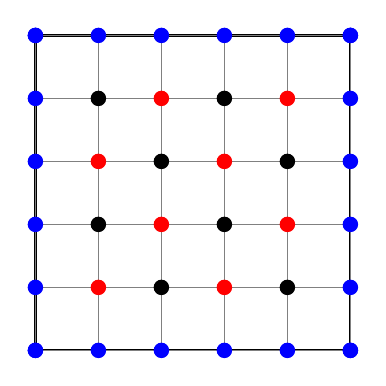
\begin{tikzpicture}[scale=4]

    % Draw square and grid
    \draw[thick] (0,0) rectangle (1,1);
    \draw[step=0.2, gray, thin] (0,0) grid (1,1);

    % Interior points (red-black pattern)
    \foreach \i in {1,...,4} {
        \foreach \j in {1,...,4} {
            \pgfmathparse{mod(\i+\j,2)==0 ? 1 : 0}
            \ifnum\pgfmathresult=1
                \fill[red] ({\i*0.2},{\j*0.2}) circle (0.7pt);
            \else
                \fill[black] ({\i*0.2},{\j*0.2}) circle (0.7pt);
            \fi
        }
    }

    % Boundary points (blue)
    \foreach \x in {0,0.2,...,1}
        \foreach \y in {0,1}
            \fill[blue] (\x,\y) circle (0.7pt);

    \foreach \y in {0,0.2,...,1}
        \foreach \x in {0,1}
            \fill[blue] (\x,\y) circle (0.7pt);

\end{tikzpicture}
\caption{Red--black ordering of interior grid points for Gauss--Seidel iteration, with boundary points shown in blue.}
\label{fig:redBlackGrid}
\end{figure}
In the red-black ordering, the red nodes are updated before the black nodes. Since the red nodes are adjacent to only black nodes, if all the red nodes are updated first, they will use only old data from the black nodes. In addition, when the black nodes are updated, which are only adjacent to red nodes, they will use only new data from the red nodes. The algorithm fo updating one step of Gauss-Seidel method for the model problem is below.
\begin{algorithm}[H]
\caption{One Gauss-Seidel iteration for the 2D Poisson equation}
\label{alg:oneStepGSPoisson}

\begin{algorithmic}[1]
\For{all notes $i,j$ that are red}
        \State {%\footnotesize
        $u_{i,j}^{(m+1)} = \dfrac{1}{4}\Big(
        u_{i+1,j}^{(m)} + u_{i-1,j}^{(m)}$}
        \Statex {%\footnotesize
        $\qquad \qquad +\, u_{i,j+1}^{(m)} + u_{i,j-1}^{(m)}
        - h^2 f_{i,j}\Big)$}    
\EndFor
\For{all notes $i,j$ that are black}
        \State {%\footnotesize
        $u_{i,j}^{(m+1)} = \dfrac{1}{4}\Big(
        u_{i+1,j}^{(m+1)} + u_{i-1,j}^{(m+1)}$}
        \Statex {%\footnotesize
        $\qquad \qquad +\, u_{i,j+1}^{(m+1)} + u_{i,j-1}^{(m+1)}
        - h^2 f_{i,j}\Big)$}    
\EndFor
\end{algorithmic}
\end{algorithm}
Note that in Algorithm~\ref{alg:oneStepGSPoisson}, the nodes of the same color can be updated in parallel, independent of each other. 
\subsection{Successive Overrelaxation}
This method is referred as SOR($\omega$), where $\omega$ is the relaxation parameter. The idea of this method is to improve the iteration in Gauss–Seidel method by taking an appropriate weighted average of the $x_j^{(m+1)}$ and $x_j^{(m)}$
\begin{align}
    x_{j}^{(m+1)} = (1-\omega)x_{j}^{(m)} + \omega x_{j}^{(m+1)}.
\end{align}
This leads to the following algorithm.
\begin{algorithm}[H]
\caption{One step of SOR($\omega$) method}
\label{alg:oneSOR}
\begin{algorithmic}[1]
\For{$i = 1$ to $n$}
    \State {%\footnotesize
    $x_{j}^{(m+1)} = (1-\omega) x_{j}^{(m)}$} +
    \Statex {%\footnotesize
    $\qquad +\displaystyle\dfrac{\omega}{a_{jj}}\left(b_j - \sum_{k=1}^{j-1} a_{jk} x_k^{(m+1)} -\sum_{k=j+1}^{n} a_{jk} x_k^{(m)} \right)$}
\EndFor
\end{algorithmic}
\end{algorithm}
As before, we want to find rewrite this method in terms of the general fixed-point iteration in~\eqref{eq:FPI}. We can rearrange the equation in Algorithm~\ref{alg:oneSOR} to get
\begin{align}
    a_{jj}x_j^{(m+1)} +  &\omega \sum_{k=1}^{j-1}a_{jk}x_k^{(m+1)}=(1-\omega)a_{jj}x_j^{(m)}, \notag\\
    &-\omega \sum_{k=j+1}^n a_{jk}x_k^{(m)} + \omega b. 
\end{align}
Again, in terms notation in~\eqref{eq:split} and~\eqref{eq:splitI}, it can be rewritten as
{\small
\begin{align}
    \mathbf{(D-\omega\tilde{L})} \mathbf{x}^{(m+1)} = \Big((1-\omega)\mathbf{D} + \omega\mathbf{\tilde{U}}\Big) \mathbf{x}^{(m)} + \omega\mathbf{b}. 
\end{align}
}
Thus
\begin{align}
    \mathbf{x}^{(m+1)} &= \mathbf{(D-\omega\tilde{L})}^{-1}\Big((1-\omega)\mathbf{D} + \omega\mathbf{\tilde{U}}\Big) \mathbf{x}^{(m)} \notag \\
    &+ \omega\mathbf{(D-\omega\tilde{L})}^{-1} \mathbf{b}.
\end{align}
Or equivalently,
\begin{align}
    \mathbf{x}^{(m+1)} &= \mathbf{(I-\omega L)}^{-1}\Big((1-\omega)\mathbf{I} + \omega\mathbf{U} \Big) \mathbf{x}^{(m)} \notag \\
    &+ \omega\mathbf{(I-\omega L)}^{-1} \mathbf{D}^{-1} \mathbf{b}.
\end{align}
Thus, this defines a fixed-point iteration for SOR($\omega$) method (the subscripit $\text{SOR($\omega$)}$ is used to indicate these matrices for SOR($\omega$)).
\begin{align}
    \mathbf{x}^{(m+1)} = \mathbf{R_{\text{SOR($\omega$)}}}\mathbf{x}^{(m)} + \mathbf{c_{\text{SOR($\omega$)}}}, \label{eq:FPISOR}
\end{align}
where the formula for $\mathbf{R_{\text{SOR($\omega$)}}}$ and $\mathbf{c_{\text{SOR($\omega$)}}}$ are given by
\begin{subequations}
\begin{align}
    & \mathbf{R_{\text{SOR($\omega$)}}} = \mathbf{(I-\omega L)}^{-1}\Big((1-\omega)\mathbf{I} + \omega\mathbf{U} \Big) ,\\ 
    & \mathbf{c_{\text{SOR($\omega$)}}} = \omega \mathbf{(I-L)^{-1}D^{-1}b}.
\end{align}
\end{subequations}
The relaxation factor $\omega$ is generally in the range $0<\omega<1$ and is usually is divided into three cases: $\omega=1$ is is equivalent to the Gauss–Seidel method,
$\omega<1$ is called underrelaxation, and $\omega>1$ is called overrelaxation. The choice of $\omega$ can significantly improve the convergence rate of the method. We will disscuss the optimal value for $\omega$ in the following section.
Returning to our model problem, there is a little change in the algorithm as for Gauss-Seidel method. Again, we will use sill red-black order to update the grid points. The SOR($\omega$) algorithm for model problem is given as follows.
\begin{algorithm}[H]
\caption{One SOR($\omega$) iteration for the 2D Poisson equation}
\label{alg:oneStepSORPoisson}

\begin{algorithmic}[1]
\For{all notes $i,j$ that are red}
        \State {%\footnotesize
        $u_{i,j}^{(m+1)} = (1-\omega) \, u_{ij}^{(m)}$}
        \Statex {%\footnotesize
        $ \qquad \qquad \qquad + \, \dfrac{\omega}{4}\Big(
        u_{i+1,j}^{(m)} + u_{i-1,j}^{(m)}$}
        \Statex {%\footnotesize
        $\qquad \qquad \qquad +\, u_{i,j+1}^{(m)} + u_{i,j-1}^{(m)}
        - h^2 f_{i,j}\Big)$}    
\EndFor
\For{all notes $i,j$ that are black}
        \State {%\footnotesize
        $u_{i,j}^{(m+1)} = (1-\omega) \, u_{ij}^{(m)}$}
        \Statex {%\footnotesize
        $ \qquad \qquad \qquad + \, \dfrac{\omega}{4}\Big(
        u_{i+1,j}^{(m+1)} + u_{i-1,j}^{(m+1)}$}
        \Statex {%\footnotesize
        $\qquad \qquad \qquad + \, u_{i,j+1}^{(m+1)} + u_{i,j-1}^{(m+1)}
        - h^2 f_{i,j}\Big)$}   
\EndFor
\end{algorithmic}
\end{algorithm}
With a suitable choice of $\omega$, which will be discussed in the next section, the Algorithm~\ref{alg:oneStepSORPoisson} gives a better convergence rate for the model problem, and again, grid nodes of the same color can be updated independently. The implementation of the parallel solvers for the model problem will be carried out based on this algorithm.
\subsection{Convergence of Jacobi's, Gauss-Seidel, and SOR($\omega$) Methods on the Poisson's Model Problems in Two Dimensions}
This section summarizes the convergence rates of the methods discussed above. For a more detailed analysis, see \cite{demmel1997,varga1962}. Recall that the convergence rate of the fixed-point iteration~\eqref{eq:FPI} depends on the spectral radius of the matrix $\mathbf{R}$. Thus, the convergence rate for Jacobi's, Gauss-Seidel, and SOR($\omega$) methods for the model problem~\eqref{eq:poisson2d} depends on the eigenvalues of matrices $\mathbf{R}_{J}$, $\mathbf{R}_{\text{GS}}$, and $\mathbf{R}_{\text{SOR($\omega$)}}$, respectively.

For the Jacobi's method, the eigenvalues of the matrix $\mathbf{R}_{J}$ for the model problem are given by $1-\lambda_{ij}/4$, where $\lambda_{ij}/4$ is given by
\begin{align}
    \lambda_{i,j}=4-2\left(\cos\left( \dfrac{\pi i}{N+1} \right) + \cos\left( \dfrac{\pi j}{N+1} \right) \right)
\end{align}
The spectral radius $\rho(\mathbf{R}_J)$ is the larges values among $|1-\lambda_{ij}/4|$, namely,
{\small
\begin{align}
    \rho(\mathbf{R}_J) =  |1-\lambda_{1,1}/4|=|1-\lambda_{N,N}/4|=\cos\left( \dfrac{\pi}{N+1} \right).
\end{align}
}
Note that
\begin{align}
    \cos\left( \dfrac{\pi}{N+1}  \right) \approx 1 - \dfrac{\pi^2}{2(N+1)^2}, \quad N\to \infty. 
\end{align}
Thus, (recall that $n=N^2$)
\begin{align}
    \rho(\mathbf{R}_J) = 1-\mathcal{O}\left( \dfrac{1}{N^2} \right) = 1-\mathcal{O}\left( \dfrac{1}{n} \right).
\end{align}
Consequently, as $N$ grows, the spectral radius $ \rho(\mathbf{R}_J)$ approaches 1 quadratically in terms of $N$, leading to a significantly large number of iterations needed for the method to converge to the solution. In fact, the number of iterations is proportional to the number of unknowns $n$. In addition, each iteration cost $\mathcal{O}(n)$. Thus the tocal cost for this method is $\mathcal{O}(n^2)$. This explains the time complexity for Jacobi’s method in Table~\ref{tab:summarySolvers}.

For the Gauss-Seidel method with the red-black ordering, the spectral radius of $\mathbf{R}_{\text{GS}}$ is given by
{
\begin{align}
    \rho(\mathbf{R}_{\text{GS}}) = \rho(\mathbf{R}_{\text{J}})^2 &=  \cos^2 \left( \dfrac{\pi}{N+1}  \right) \\
    &\approx 1 - \dfrac{\pi^2}{(N+1)^2}. \notag
\end{align}
}
In other words, one Gauss–Seidel iteration decreases the error as much as two Jacobi iterations. Thus, Gauss–Seidel method is as twice as fast as of that of Jacobi's method. However, the total cost for Gauss-Seidel is still $\mathcal{O}(n^2)$. This also explains the time complexity for the Gauss–Seidel method in Table ~\ref{tab:summarySolvers}.; since it is only twice as fast as Jacobi, it still has the same complexity in the $\mathcal{O}(\cdot)$ sense.

For the SOR($\omega$) method for the model problem, one can show that for the relaxation parameter $\omega$ satisfies
\begin{align}
    1 <  \omega = \dfrac{2}{1+\sin \Big ( \pi /(N+1) \Big)} <2 \label{eq:optOmega}
\end{align}
then
{\small
\begin{align}
    \rho( \mathbf{R}_{\text{SOR($\omega$)}} ) = \dfrac{\cos^2\Big(\dfrac{\pi}{N+1} \Big)}{\left( 1+\sin\Big(\dfrac{\pi}{N+1} \Big) \right)^2} . 
\end{align}
This gives,
\begin{align}
    \rho( \mathbf{R}_{\text{SOR($\omega$)}} )\approx 1-\dfrac{2\pi}{N+1}, \quad N \to \infty.
\end{align}
}
Thus, the number of iterations grow like $\mathcal{O}(N)=\mathcal{O}(\sqrt{n})$ as in contrast to Jacobi and Gauss-Seidel methods. The value of $\omega$ given in~\eqref{eq:optOmega} is the optimal value for SOR($\omega$). With this choice of $\omega$, this method is approximately $N$ times faster than Jacobi’s or the Gauss-Seidel method. Thus, it reduces the complexity of SOR($\omega$) from $\mathcal{O}(n^2)$ to $\mathcal{O}(n^{3/2})$, as shown in Table~\ref{tab:summarySolvers}.
% \begin{figure}[htb]
%  \centering
%  % \includegraphics[width=0.6\linewidth,trim={22.0cm 15.0cm 22.0cm 15.0cm},clip,angle=0,origin=c]{appelo-fig5.png}
%  \includegraphics[width=0.7\linewidth,
%  trim={0.1cm 0.1cm 0.1cm 0.1cm},
%  clip,
%  angle=0,
%  origin=c]
%  {grid.png}
%  \caption{Overset grid with Dirichlet boundary condition imposed on the cylinder (blue circle) and RBCs on all boundaries of the square. \label{fig:mesh}}
% \end{figure}
\section{Numerical Results}\label{sec:results}
This section presents the numerical results for the parallel Poisson solver, which is based on the red-black ordering SOR($\omega$) method as discussed in Algorithm~\ref{alg:oneStepSORPoisson} above. The forcing term $f(x,y)$ in the equation~\eqref{eq:poisson2d} is defined as
\begin{align}
f(x,y) &= \dfrac{10\lambda}{\pi} e^{-\lambda^2\left( (x-0.5)^2 + (y-0.5)^2 \right)} \notag \\ & -\dfrac{10\lambda}{\pi} e^{-\lambda^2\left( (x-0.25)^2 + (y-0.25)^2 \right)},
\end{align}
% In this section, we illustrate the numerical results for the parallel solver for Poisson's equation based on Algorithm~\ref{alg:oneStepSORPoisson}. 
% The function $f(x,y)$ in\eqref{eq:poisson2d} is
% {\small
% \begin{align}
%     f(x,y)= \dfrac{10\lambda}{\pi}\left[ e^{-\lambda^2\left( (x-1)^2 + y^2 \right)} + e^{-\lambda^2\left( (x+1)^2 + y^2 \right)}\right]
% \end{align}
% }
where the value of $\lambda=100$, with the four boundary sides of $u$ is zeros, i.e., $g=0$. Here, the two terms represent approximations of a Dirac delta point source of strength 10 at $(0.5,0.5)$ and a sink at $(0.25,0.25)$. This is a model of a plate with four sides held at a fixed temperature. The value of $\lambda$ controls how narrow or wide the approximate Dirac delta is spread, with larger values being more narrow, and approaching the true Dirac delta as $\lambda\to \infty$. The plot of the forcing $f(x,y)$ and the computed solution $u(x,y)$ (solved in MATLAB) is demonstrated in Figure~\ref{fig:forcing_computed_solution}.
\begin{figure}[H]
 \centering 
 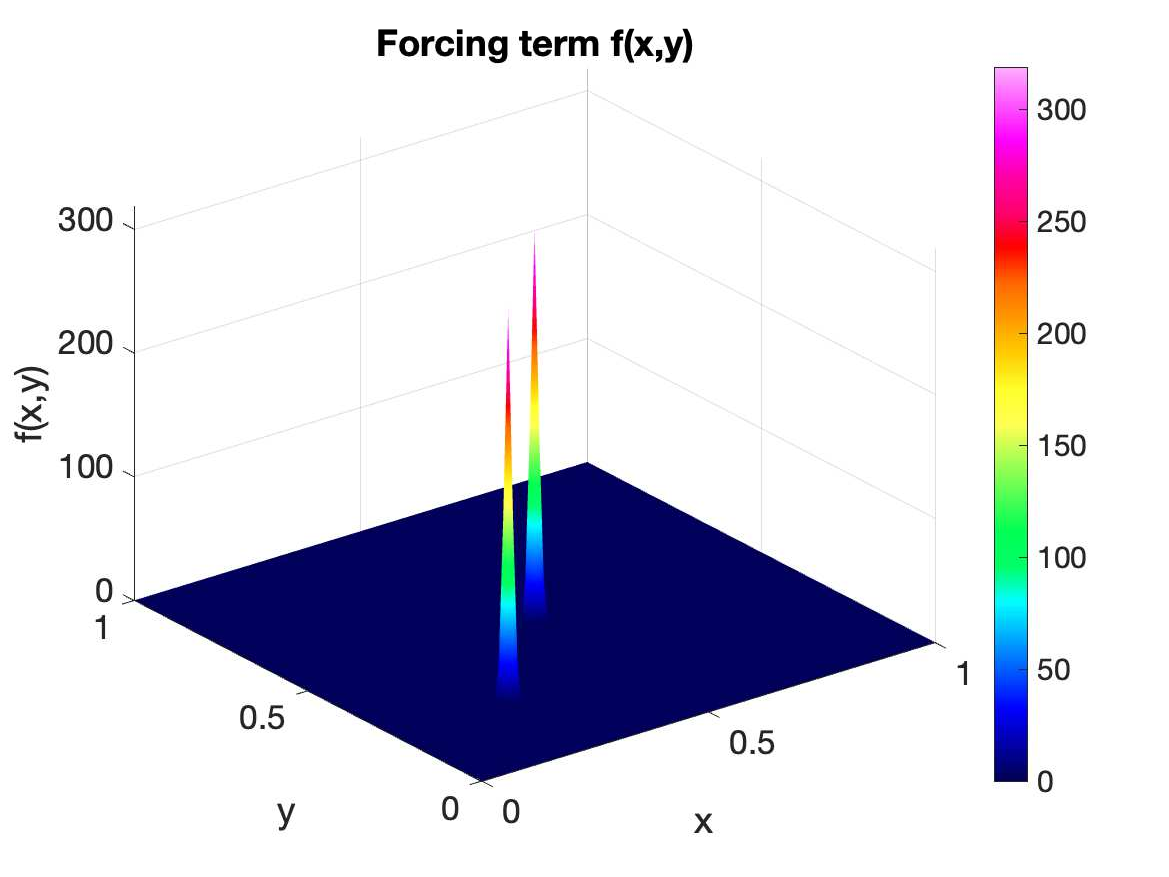
\includegraphics[width=0.9 \linewidth,
 trim={0.0cm 0.0cm 0.0cm 0.0cm},
 clip,
 angle=0,
 origin=c]
 {fig/forcing.pdf} \quad
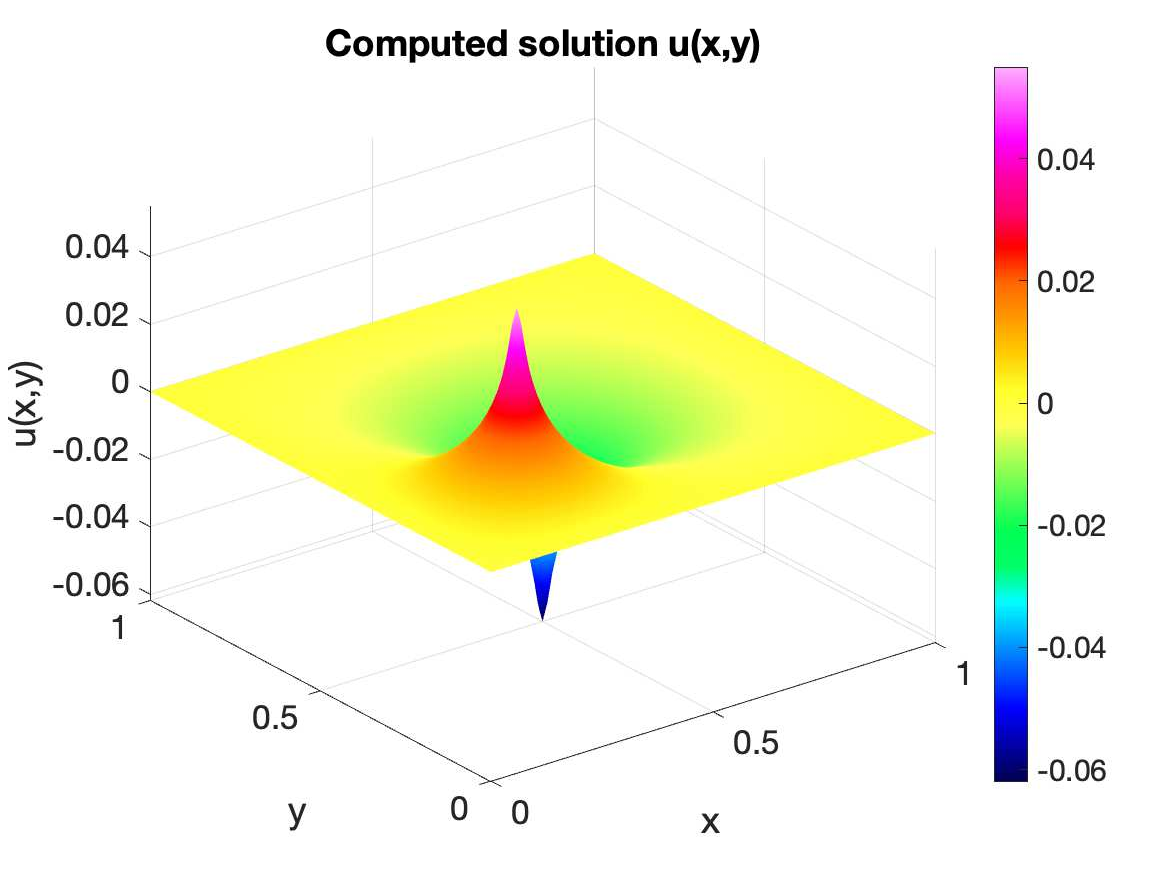
\includegraphics[width=0.9 \linewidth,
 trim={0.0cm 0.0cm 0.0cm 0.0cm},
 clip,
 angle=0,
 origin=c]
 {fig/computed_solution.pdf}
 \caption{The forcing $f(x,y)$ and the computed solution $u(x,y)$. \label{fig:forcing_computed_solution}}
\end{figure}

To determine the convergence of the iterative solver, we will use the common stopping criterion based on the residual $r_{ij}$, which is defined as follows.
\begin{align}
    r^{(m)}_{ij} \stackrel{\mathrm{def}}{=} &u^{(m)}_{i+1,j}+u^{(m)}_{i-1,j} + u^{(m)}_{i,j+1}+u^{(m)}_{i,j-1} \notag \\
    &- 4u^{(m)}_{i,j} - h^2 f_{ij}.
\end{align}
Convergence is reached when the maximum absolute value of the residual (the $L_\infty$ norm), scaled by $1/h$, is below a specified tolerance $\epsilon$. For the numerical results presented in this section, we choose $\epsilon=10^{-10}$, thus the stopping condition is
\begin{equation}\dfrac{1}{h}\max_{i,j} |r^{(m)}_{ij}| < 10^{-10}.\end{equation}
In all cases, the program takes four arguments so that the program will be executed like this:
\begin{align*}
    \text{\$ ./\textit{executable} 128 1.8 1e-10 20000}
\end{align*}
where \textit{executable} is the name of the executable, e.g., \textit{poisson2d\_cuda} for the CUDA test case, the number of grid points in each direction $N=128$, giving $n=N^2=16384$ grid points in total. The overrelaxation parameter is $\omega=1.8$ and the convergence tolerance is $\epsilon=10^{-10}$.
Note that the numerical results presented here were tested with the optimal value of $\omega$ given in Equation~\eqref{eq:optOmega}. If the input $\omega=2.0$, then it will convert to the optimal value for $\omega$. The maximum iterations is $K=20000$.


\subsection{Solver verification}
The serial and MPI codes are verified with two exact solutions on the unit square; the forcing is $f=u_{xx}+u_{yy}$ and the boundary values are $g=u$:
\begin{align*}
  u_{\text{poly}} &= p(x)\,q(y), \\
  p(x) &= 0.5+0.7x-0.3x^2-0.2x^3, \\
  q(y) &= 0.75-0.45y-0.3y^2+0.25y^3, \\
  u_{\text{gauss}} &= e^{-2(x-0.3)^2}\,e^{-2(y-0.7)^2},
\end{align*}
The fourth derivatives of $u_{\text{poly}}$ vanish, so the 5-point stencil is exact and the error comes only from the stopping tolerance. Table~\ref{tab:verification} shows the maximum errors for $\omega$ optimal and $\epsilon=10^{-10}$.
\begin{table}[H]\footnotesize
\setlength{\tabcolsep}{3pt}
\begin{center}
\begin{tabular}{rrcrcc}
\toprule
 & \multicolumn{2}{c}{poly} & \multicolumn{3}{c}{gauss} \\
$N$ & iter. & max error & iter. & max error & ratio \\
\midrule
16  & 77  & $6.57\cdot10^{-12}$ & 79  & $1.01\cdot10^{-3}$ & -- \\
32  & 149 & $7.66\cdot10^{-12}$ & 153 & $2.69\cdot10^{-4}$ & 3.75 \\
64  & 294 & $7.30\cdot10^{-12}$ & 303 & $6.95\cdot10^{-5}$ & 3.88 \\
128 & 587 & $6.27\cdot10^{-12}$ & 603 & $1.77\cdot10^{-5}$ & 3.94 \\
\bottomrule
\end{tabular}
\caption{Verification: iterations and maximum errors for the exact solutions. \label{tab:verification}}
\end{center}
\end{table}
The polynomial solution is computed to the level of the tolerance, and the error ratio for the Gaussian solution approaches 4, i.e., second-order convergence. The MPI code gives the same iterations, residuals and errors as the serial code for $n_p=1,2,3,4$ (script \texttt{run\-Baseline.sh}).

\subsection{Parallel using MPI results}
The timings in this and the next subsection were measured with an earlier version of the code, in which the forcing was centered at $(\pm1,0)$. The time per iteration does not depend on the forcing, but the number of iterations, and hence the total runtime, does.
We present the runtimes and speedups when we implement the SOR($\omega$) methods parallelized using only MPI.

\begin{figure}[H]
 \centering 
 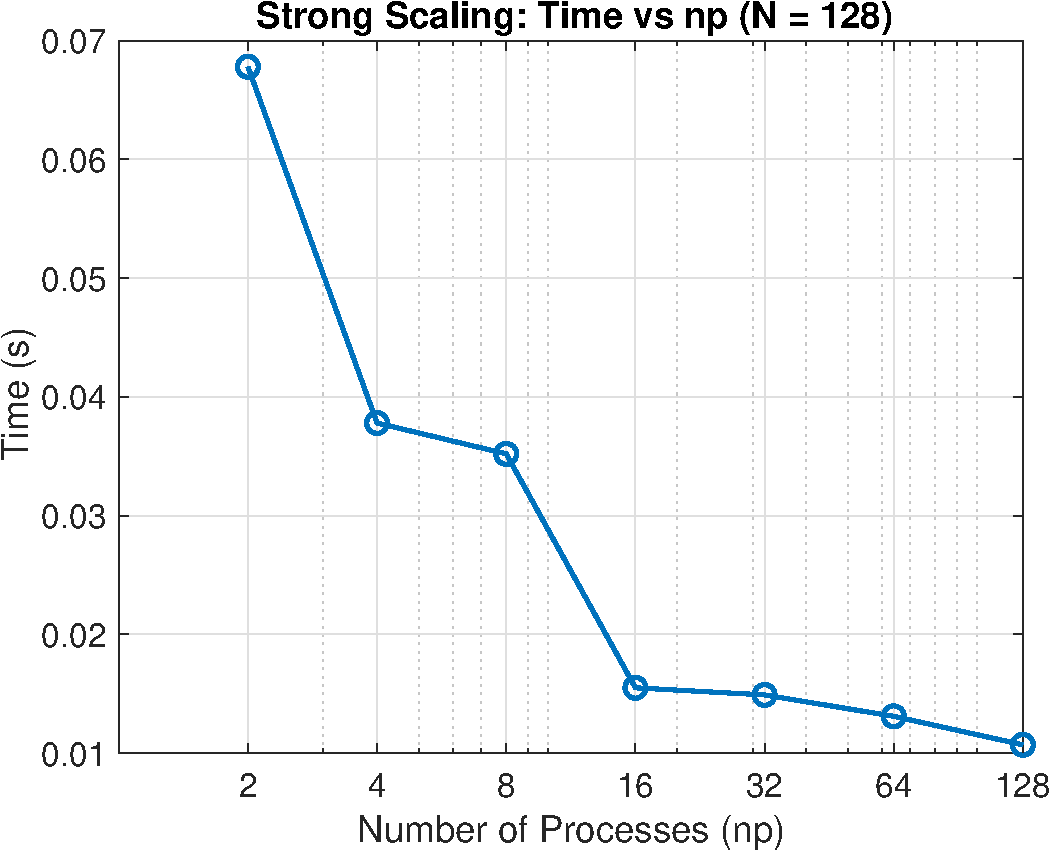
\includegraphics[width=0.9 \linewidth,
 trim={0.0cm 0.0cm 0.0cm 0.0cm},
 clip,
 angle=0,
 origin=c]
 {fig/strong_scaling_time_N_128.pdf} \quad
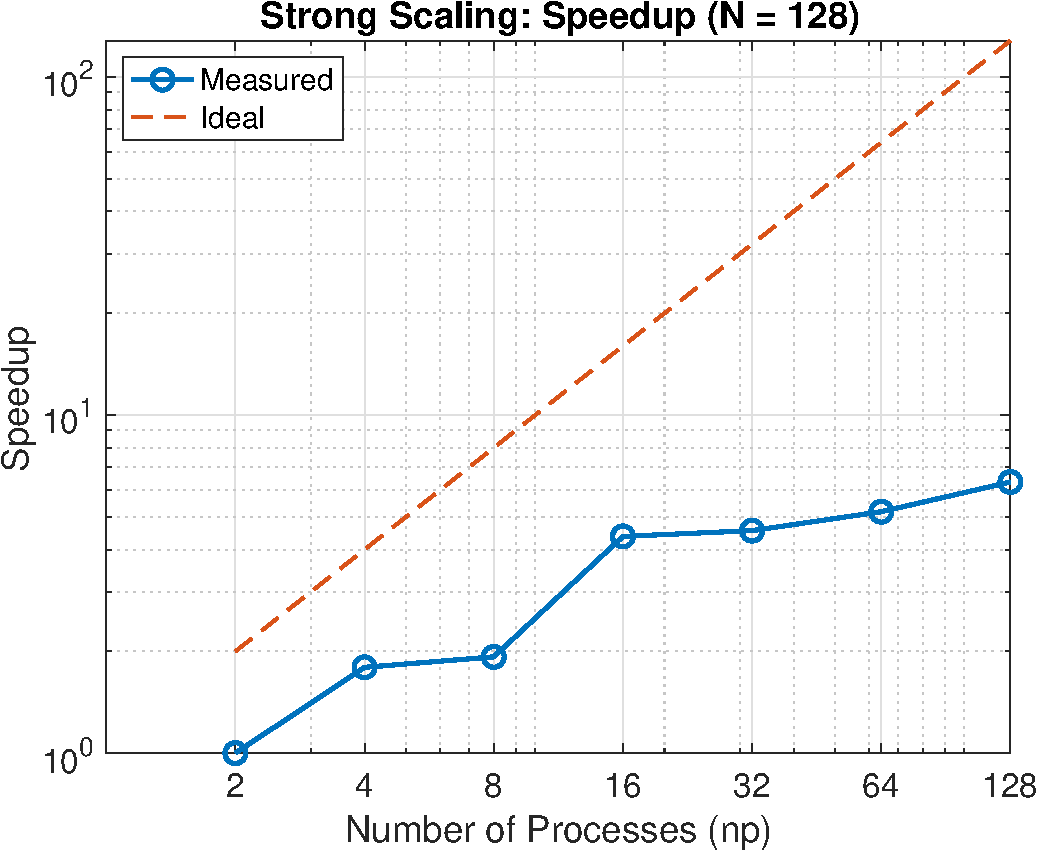
\includegraphics[width=0.9 \linewidth,
 trim={0.0cm 0.0cm 0.0cm 0.0cm},
 clip,
 angle=0,
 origin=c]
 {fig/strong_scaling_speedup_N_128.pdf}
 \caption{ The runtimes and speedups for the MPI test case with $N=128$. 
 \label{fig:strong_scaling_N_128}}
\end{figure}
 We divide the domain only in the $y$ direction. For interior ranks, i.e., ranks ranging from $1,2,\cdots,n_p-2$, there will be two halos each at each in the $y$-direction. For rank 0, we only need the halo in the uper end and for rank $n_p-1$ we only need the halo at the lower end.
At each iteration, after updating the red grid nodes in Algorithm ~\ref{alg:oneStepSORPoisson}, we need to exchange data among different ranks, since we need the updated value at the boundary for updating the black nodes. Similarly, after updating the black grid nodes, we again need to exchange the data among different ranks to update the value of the boundary points for the next iteration. Thus, each iteration requires two communications, which is somewhat expensive since the communication is the bottleneck in the runtime.
\paragraph{Strong Scaling test.}
For a strong scaling parallel test case, we ran the parallel solver using only the MPI version and tested for four different values of $N$ with $N=128, 256, 512, 1024$. The runtime and the speedup are illustrated in Figures~\ref{fig:strong_scaling_N_128},~\ref{fig:strong_scaling_N_256},~\ref{fig:strong_scaling_N_512}, and~\ref{fig:strong_scaling_N_1024}, respectively. We observe that in all cases, as we increase the number of processes, the runtime decreases, which indicates that we have gained some speedup, as we should expect. 
\begin{figure}[H]
 \centering
  
 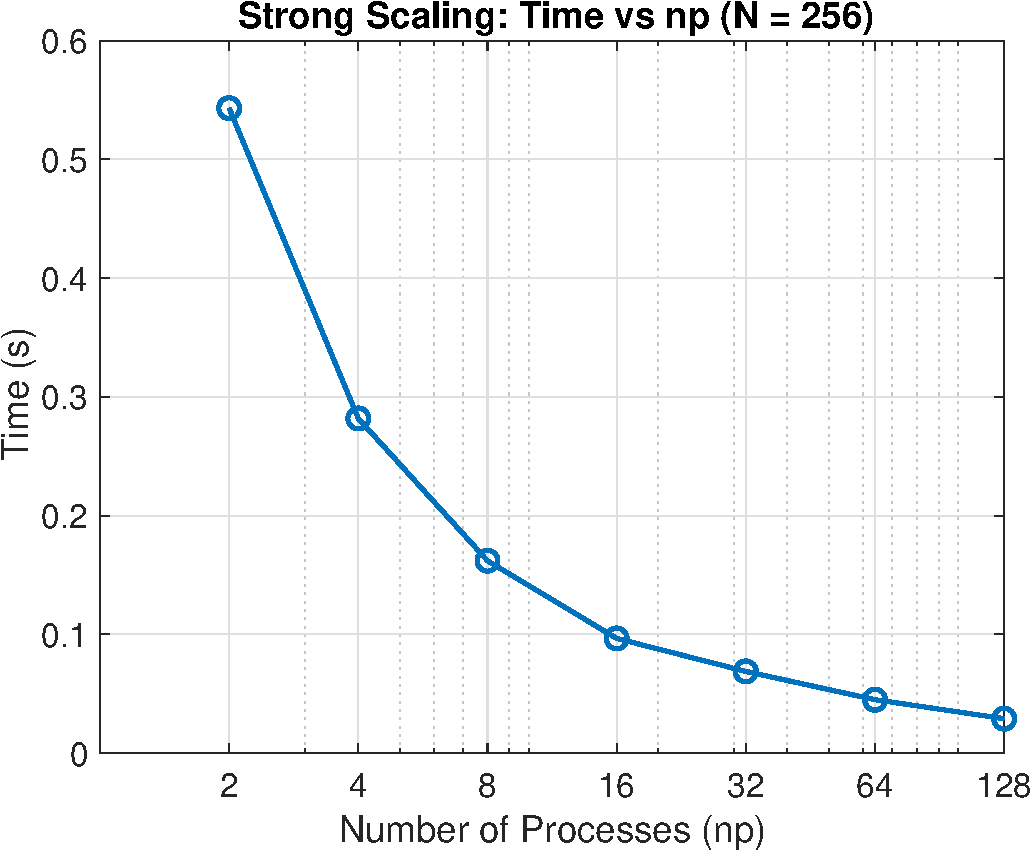
\includegraphics[width=0.9\linewidth,
 trim={0.0cm 0.0cm 0.0cm 0.0cm},
 clip,
 angle=0,
 origin=c]
 {fig/strong_scaling_time_N_256.pdf} \quad
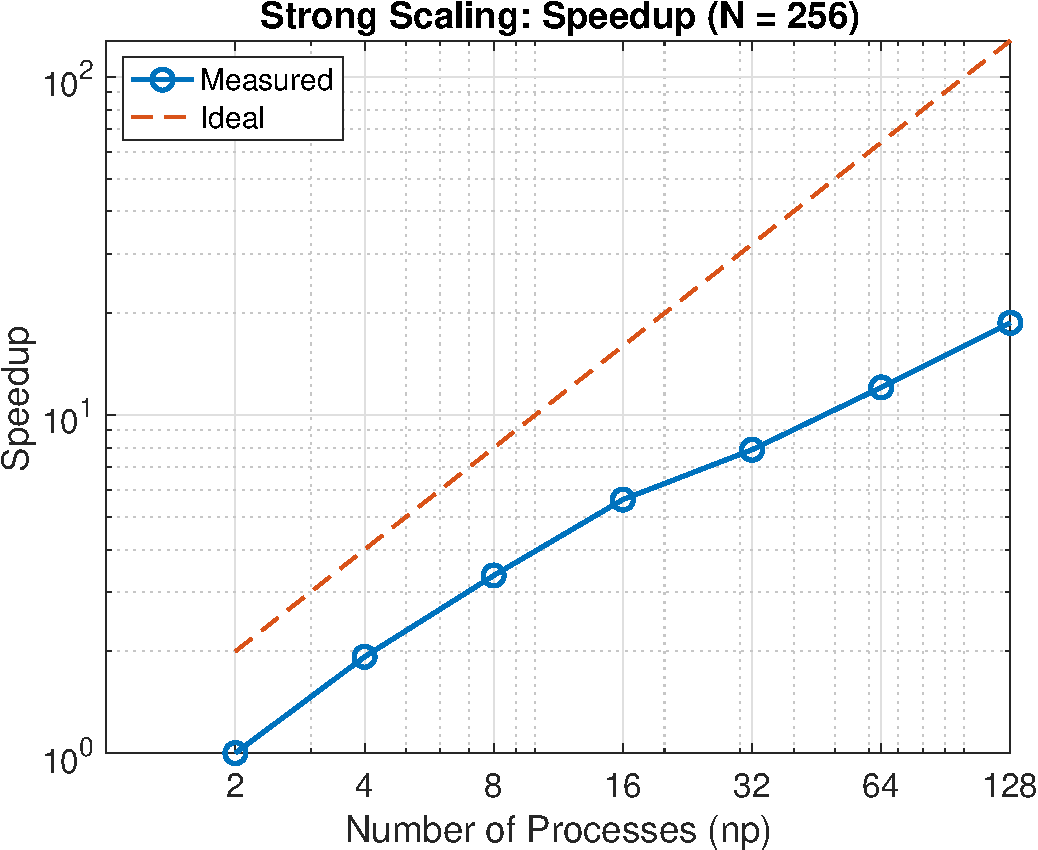
\includegraphics[width=0.9\linewidth,
 trim={0.0cm 0.0cm 0.0cm 0.0cm},
 clip,
 angle=0,
 origin=c]
 {fig/strong_scaling_speedup_N_256.pdf}
 \caption{The runtimes and speedups for the MPI test case with $N=256$. \label{fig:strong_scaling_N_256}}
\end{figure}

When the number of processes is small, i.e., when $n_p=2,4,8, 16$, doubling the number of processes leads to a reduction in runtime roughly by half, which is the optimal behavior we expect. Except for the case $N=128$, when increasing from $n_p=4$ to $n_p=8$ the runtime reduction is negligible. Then it dropped by half when the number of ranks increased from 8 to 16. The behavior of the runtime in this case is unclear. It may be possible that, in this case, since the problem size is small the overhead cost is dominated by the communication time.


\begin{figure}[H]
 \centering
  
 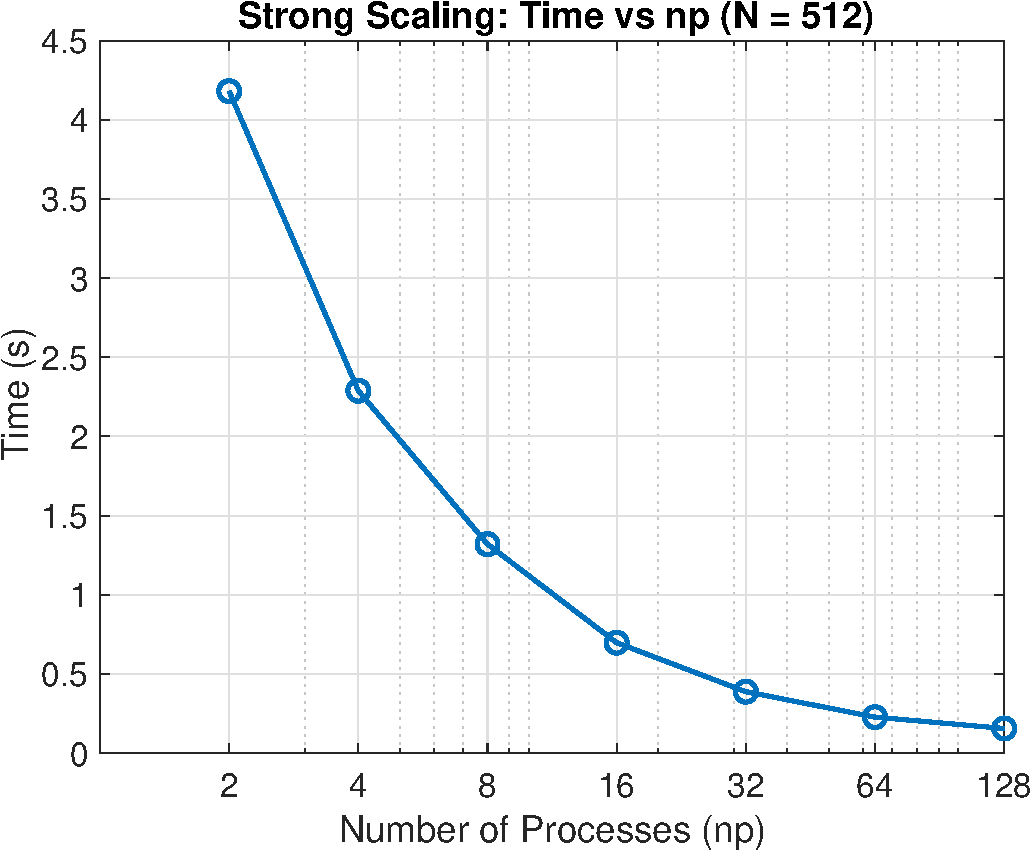
\includegraphics[width=0.9\linewidth,
 trim={0.0cm 0.0cm 0.0cm 0.0cm},
 clip,
 angle=0,
 origin=c]
 {fig/strong_scaling_time_N_512.pdf} \quad
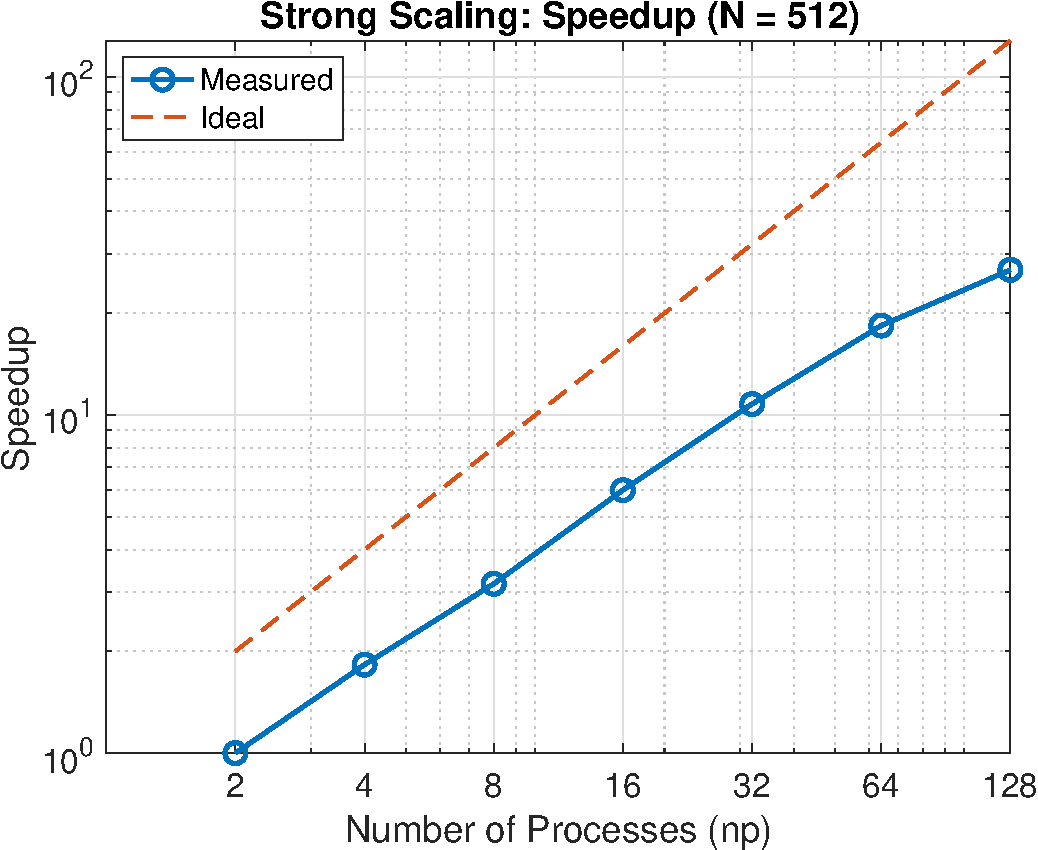
\includegraphics[width=0.9\linewidth,
 trim={0.0cm 0.0cm 0.0cm 0.0cm},
 clip,
 angle=0,
 origin=c]
 {fig/strong_scaling_speedup_N_512.pdf}
 \caption{The runtimes and speedups for the MPI test case with $N=512$. \label{fig:strong_scaling_N_512}}
\end{figure}
When the number of processes becomes large, i.e $n_p=32,64,128$, the communication cost becomes dominant, especially for the case $n_p=128$. We do not see the ideal case where the runtime is reduced by half.
We also see good scaling and speed up when the problem sizes get larger, especially in the case $N=512$ and $N=1024$. It seems that the runtime is reduced by half as the number of processes is doubled. The speedup curves are very aligned with the ideal curves in these cases, except for the case $n_p=128$, where the communication cost becomes dominant. Thus, it indicates the method is strongly scalable for large-scale problems. 
\begin{figure}[H]
 \centering
 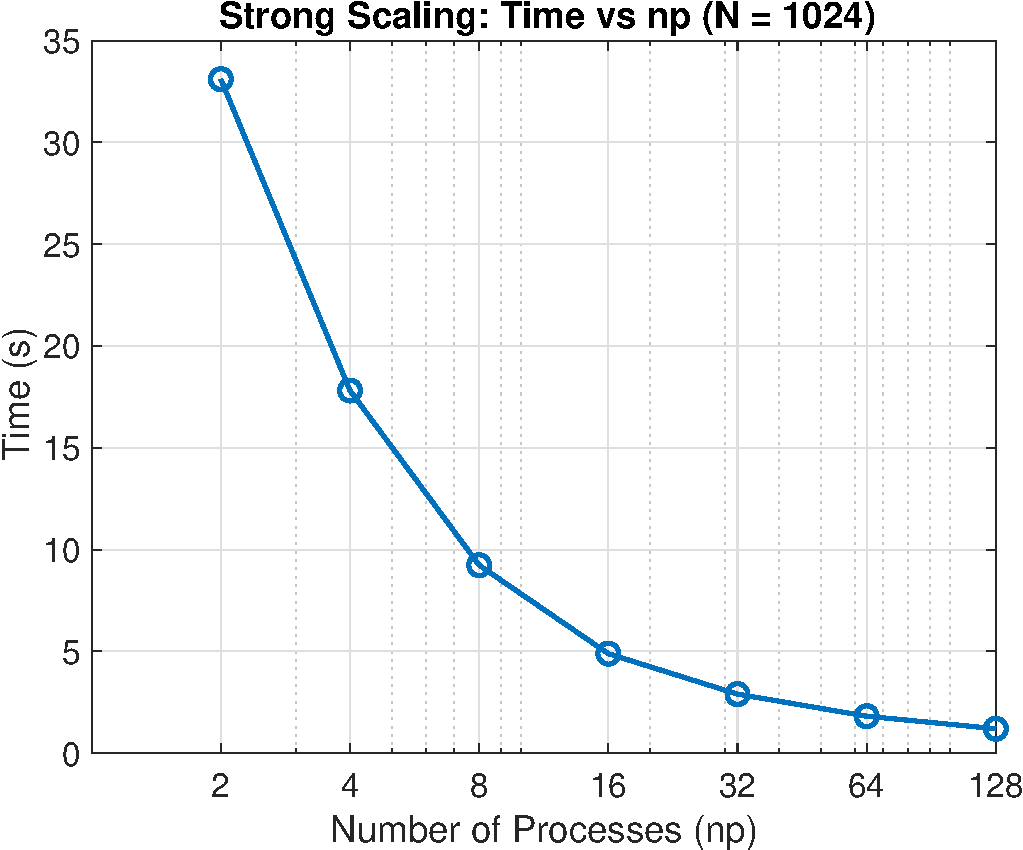
\includegraphics[width=0.9\linewidth,
 trim={0.0cm 0.0cm 0.0cm 0.0cm},
 clip,
 angle=0,
 origin=c]
 {fig/strong_scaling_time_N_1024.pdf} \quad
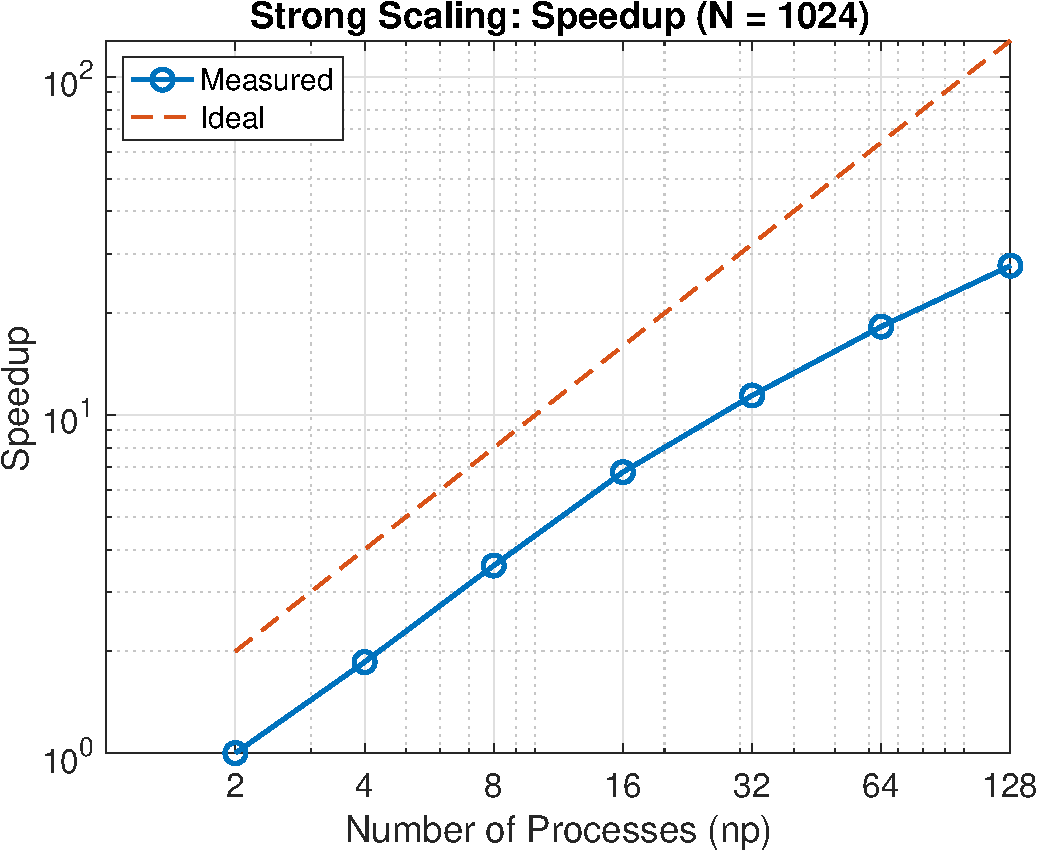
\includegraphics[width=0.9\linewidth,
 trim={0.0cm 0.0cm 0.0cm 0.0cm},
 clip,
 angle=0,
 origin=c]
 {fig/strong_scaling_speedup_N_1024.pdf}
 \caption{The runtimes and speedups for the MPI test case with $N=1024$. \label{fig:strong_scaling_N_1024}}
\end{figure}

 
\paragraph{Weak Scaling test.}

For the weak scaling test, since the problem size is $n=N^2$, doubling $N$ results in an increase of 4 times in the problem size. In addition, the number of iterations also scales with $N$ as $N$ grows. Thus, we will measure the runtime per iteration instead of the total runtime. The problem size $N$ is varied across the values 256, 512, 1024, and 2048 with the number of processes $n_p$ set to 2, 8, 32, and 128, respectively. The numerical runtime for weak scaling is illustrated in Figure~\ref{fig:weak_scaling_MPI}.
\begin{figure}[H]
 \centering 
 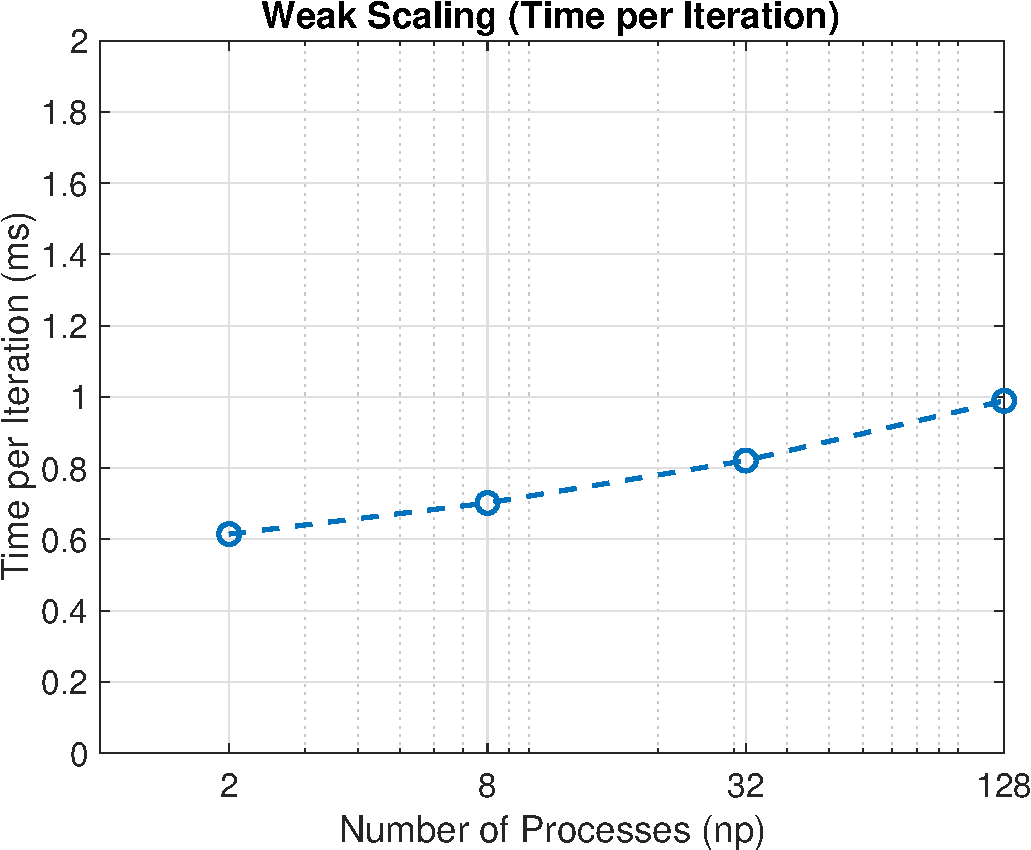
\includegraphics[width=0.9\linewidth,
 trim={0.0cm 0.0cm 0.0cm 0.0cm},
 clip,
 angle=0,
 origin=c]
 {fig/weak_scaling_runtime.pdf}
 \caption{MPI runtime performance for weak scaling in milliseconds. \label{fig:weak_scaling_MPI}}
\end{figure}
In an ideal weak-scaling case, one would expect the runtime per iteration to remain constant as the problem size increases according to the number of processes used. As illustrated in~\ref{fig:weak_scaling_MPI}, for the two-rank case, the runtime per iteration is approximately 0.6 ms. However, at 128 ranks, this increases by roughly $61\%$ to nearly 1.0 ms. While the figure seems to be small, this overhead becomes significant for large problems where a high number of iterations is required for the problem to converge, which leads to a substantial increase in total execution time. Thus, the inter-process communication between processes is still a primary bottleneck for large-scale simulations.


\subsection{Parallel using MPI + CUDA results}
We now present results for the Poisson solver using combined MPI and CUDA parallelization. The test cases utilize grid resolutions $N$ ranging in the set $\{256, 512, 1024, 2048, 4096\}$. At $N=4096$, the system involves over $n\approx 1.6 \times 10^7$ variables (more than 16 million grid points); since the SOR method scales as $\mathcal{O}(n^{3/2})$, these simulations are computationally demanding and provide a good test for our parallel. Note that for $n_p=1$, we only use CUDA parallelization, so there is no communication overhead cost in this case. Also, due to the limited number of resources and the nature of the problem, weak scaling is not tested in this section.
\begin{figure}[H]
 \centering 
 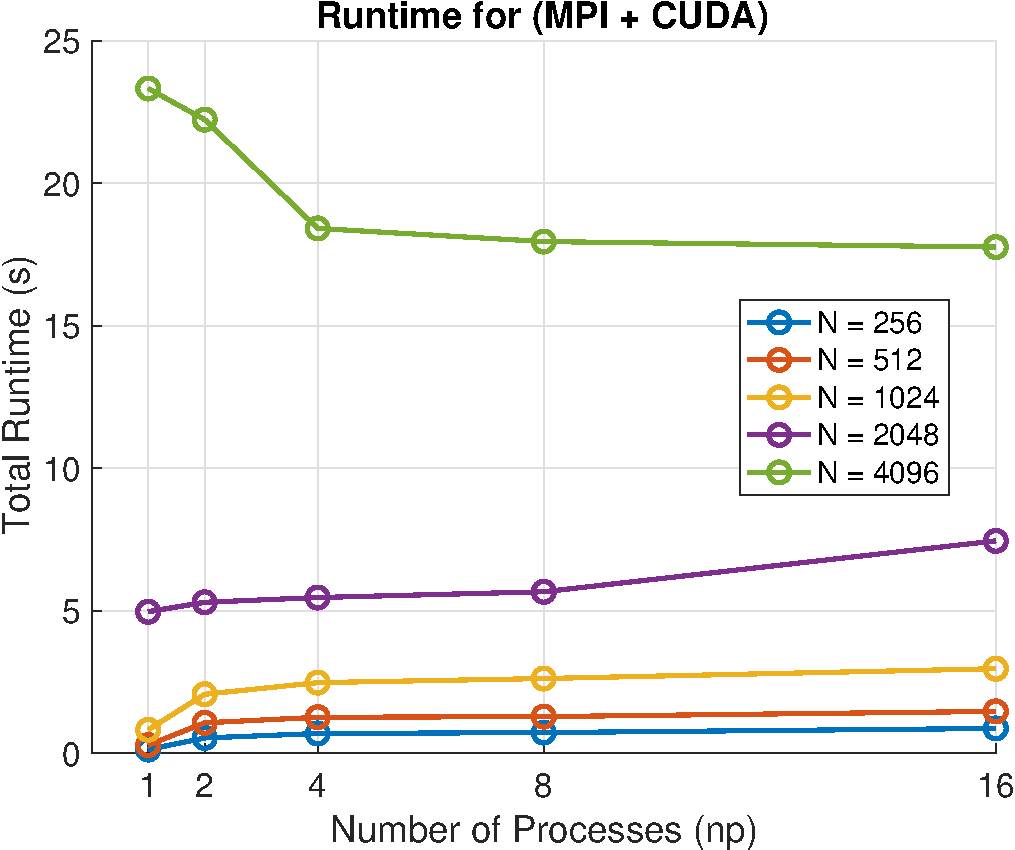
\includegraphics[width=0.9\linewidth,
 trim={0.0cm 0.0cm 0.0cm 0.0cm},
 clip,
 angle=0,
 origin=c]
 {fig/mpi_cuda_runtime.pdf}
 \caption{Execution time for the hybrid MPI-CUDA Poisson solver. \label{fig:mpi_cuda_runtime}}
\end{figure}
The runtime is plotted in Figure~\ref{fig:mpi_cuda_runtime}. As can be seen from the figure, when the problem size is small, using only a single GPU is sufficient, and increasing the number of processes did not help increase the performance at all. It is also because of the time for data to move to GPUs can cause the overhead as well as the increase in data communication among ranks. For a large problem as in the case $N=4096$, we see that increasing the number of processes leads to reducing the runtime, although it does not reduce significantly, as in the case of MPI version only. For $n_p$ increases from 1 to 4, there is a good reduction in the runtime. Then, due to the computational communication and also data migration to GPU, although the run time still reducess but the reduction is minimal.
The runtime for the case $n_p=16$ and compared with the parallel solver implemented using CUDA only is plotted in Figure~\ref{fig:mpi_cuda_compare}
\begin{figure}[H]
 \centering 
 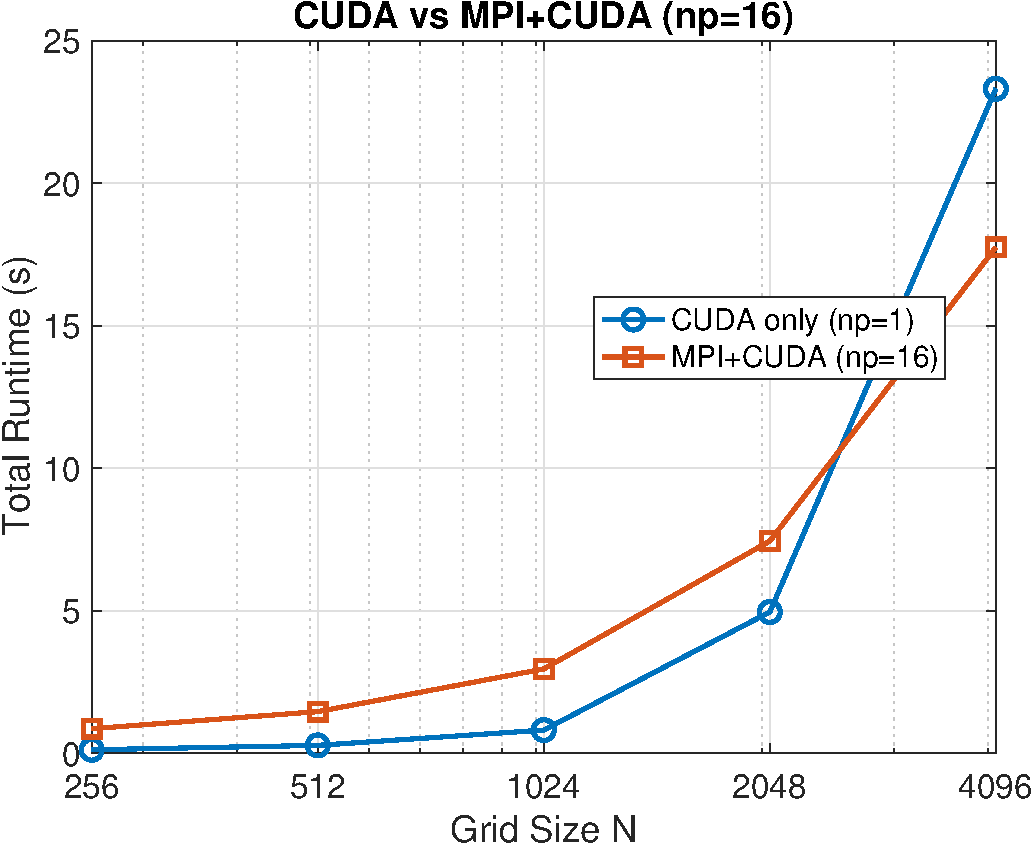
\includegraphics[width=0.9\linewidth,
 trim={0.0cm 0.0cm 0.0cm 0.0cm},
 clip,
 angle=0,
 origin=c]
 {fig/mpi_cuda_compare.pdf}
 \caption{Runtime of the MPI+CUDA solver with $n_p=16$ compared with the CUDA-only solver.}\label{fig:mpi_cuda_compare}
\end{figure}

\section{Conclusions}
This work presented parallel implementations of a Poisson solver using MPI and CUDA. We demonstrated that these methods achieve strong scalability and significant speedup, making them well-suited for high-resolution scientific simulations. In the future, we can extend this approach to 3D domains and fluid dynamics applications, such as Stokes flow. Additionally, we aim to implement more sophisticated algorithms, such as multigrid solvers and domain decomposition methods.

\textbf{Acknowledgment: This work was performed individually by me.}

\begin{thebibliography}{99}

\bibitem{adams1988}
M. F. Adams and H. F. Jordan, Is SOR color-blind?, \textit{SIAM J. Sci. Stat. Comput.}, \textbf{7} (1986), pp. 490--506.

\bibitem{brandt1977}
A. Brandt, Multi-level adaptive solutions to boundary-value problems, \textit{Math. Comp.}, \textbf{31} (1977), pp. 333--390.

\bibitem{briggs2000}
W. L. Briggs, V. E. Henson, and S. F. McCormick, \textit{A Multigrid Tutorial}, 2nd ed., SIAM, Philadelphia, 2000.

\bibitem{cooley1965}
J. W. Cooley and J. W. Tukey, An algorithm for the machine calculation of complex Fourier series, \textit{Math. Comp.}, \textbf{19} (1965), pp. 297--301.

\bibitem{demmel1993}
J. Demmel, The complexity of solving linear systems, \textit{Acta Numerica}, \textbf{2} (1993), pp. 201--272.

\bibitem{demmel1997}
J. W. Demmel, \textit{Applied Numerical Linear Algebra}, SIAM, Philadelphia, 1997.

\bibitem{gholami2016}
A. Gholami, D. Malhotra, H. Sundar, and G. Biros, FFT, FMM, or multigrid? A comparative study of state-of-the-art Poisson solvers for uniform and nonuniform grids in the unit cube, \textit{SIAM J. Sci. Comput.}, \textbf{38} (2016), pp. C280--C306.

\bibitem{hackbusch1994}
W. Hackbusch, \textit{Iterative Solution of Large Sparse Systems of Equations}, Springer, 1994.

\bibitem{hockney1988}
R. W. Hockney and J. W. Eastwood, \textit{Computer Simulation Using Particles}, Taylor \& Francis, 1988.

\bibitem{leveque}
R. J. LeVeque, \textit{Finite Difference Methods for Ordinary and Partial Differential Equations: Steady-State and Time-Dependent Problems}, SIAM, Philadelphia, 2007.

\bibitem{saad2003}
Y. Saad, \textit{Iterative Methods for Sparse Linear Systems}, 2nd ed., SIAM, Philadelphia, 2003.

\bibitem{smith1996}
B. F. Smith, P. E. Bj{\o}rstad, and W. D. Gropp, \textit{Domain Decomposition: Parallel Multilevel Methods for Elliptic Partial Differential Equations}, Cambridge University Press, 1996.

\bibitem{trefethen1997}
L. N. Trefethen and D. Bau III, \textit{Numerical Linear Algebra}, SIAM, Philadelphia, 1997.

\bibitem{trottenberg2001}
U. Trottenberg, C. W. Oosterlee, and A. Sch\"uller, \textit{Multigrid}, Academic Press, 2001.

\bibitem{varga1962}
R. S. Varga, \textit{Matrix Iterative Analysis}, Prentice-Hall, 1962.

\bibitem{young1954}
D. M. Young, Iterative methods for solving partial difference equations of elliptic type, \textit{Trans. Amer. Math. Soc.}, \textbf{76} (1954), pp. 92--111.

\bibitem{zhang1996}
J. Zhang, Acceleration of red-black Gauss-Seidel method in multigrid for Poisson equation, \textit{Appl. Math. Comput.}, \textbf{80} (1996), pp. 73--93.

\end{thebibliography} 
% ------------------------------------------------------------------------
% --------------- DO NOT EDIT THE FILE BELOW THIS LINE -------------------
% ------------------------------------------------------------------------


\end{document}
